\documentclass[12pt,letterpaper,fleqn]{article}          % fleqn: align equations left

% File produced by Jeremy West
% This file may be distributed and/or modified:
%   1. under the LaTeX Project Public License and/or
%   2. under the GNU Public License.

% Pretty much required packages for me:
\usepackage{fullpage}                                    % Use the full page
\usepackage{fontspec}
\setmainfont{baskerville}
\usepackage{amsmath}                                     % Math equations, etc.
\usepackage{graphicx}                                    % Enable images (no .eps w/o below option)
\usepackage{epstopdf}                                    % Convert .eps images on the fly
\usepackage{color}                                       % Enables colored text
\definecolor{darkblue}{rgb}{0.0,0.0,0.66}                % Custom color: dark blue
\usepackage[hyperfootnotes=false,bookmarksopen]{hyperref}% Enable hyperlinks, expand menu subtree
\hypersetup{                                             % Custom hyperlink settings
    pdffitwindow=false,                                  % true: window fit to page when opened
    pdfstartview={XYZ null null 1.00},                   % Fits the zoom of the page to 100%
    pdfnewwindow=true,                                   % Links in new window
    colorlinks=true,                                     % false: boxed links; true: colored links
    linkcolor=darkblue,                                  % Color of internal links
    citecolor=darkblue,                                  % Color of links to bibliography
    urlcolor=darkblue  }                                 % Color of external links
\usepackage{booktabs}                                    % For better tables
\newcommand{\ra}[1]{\renewcommand{\arraystretch}{#1}}    % Spacing for tables improved
\renewcommand{\arraystretch}{1.5}                        % Spaces arrays at 1.5x for readability
\usepackage{pdflscape}                                   % Use: \begin{landscape} ... \end{landscape}

% Some "optional" packages that I frequently use:
\usepackage{datetime}                                    % Custom date format for date field
\newdateformat{mydate}{\monthname[\THEMONTH] \THEYEAR}   % Defining month year date format
\usepackage[authoryear]{natbib}                          % Bibliography and citation formating
\usepackage[section]{placeins}                           % Forces floats to stay in section
\usepackage{float}                                       % Used with restylefloat
\restylefloat{figure}                                    % "H" forces a figure to be "exactly here"
\usepackage{textcomp}                                    % Supports many additional symbols
\usepackage{amsthm}                                      % Math theorems, etc.
\usepackage{amsfonts}                                    % Math fonts (e.g. script fonts)
\usepackage{amssymb}                                     % Math symbols such as infinity
\DeclareMathOperator*{\Max}{Max}                         % Better looking max function
\DeclareMathOperator*{\Min}{Min}                         % Better looking min function
\usepackage{subfig}                                      % Enables arrayed images
\usepackage{setspace}                                    % Enables custom margins, doublespacing, etc.
\usepackage{tikz}                                        % Timelines and other drawings
\usetikzlibrary{decorations}                             % Formating for Tikz


\usepackage{color}

\definecolor{mygreen}{rgb}{0,0.6,0}
\definecolor{mygray}{rgb}{0.5,0.5,0.5}
\definecolor{mymauve}{rgb}{0.58,0,0.82}
\definecolor{light-gray}{gray}{0.95}
\usepackage{listings}

\lstdefinestyle{customc}{
backgroundcolor=\color{light-gray},
  belowcaptionskip=1\baselineskip,
  breaklines=true,
  frame=single,
  xleftmargin=\parindent,
  language=C++,
  showstringspaces=false,
  basicstyle=\footnotesize\ttfamily,
  keywordstyle=\bfseries\color{green!40!black},
  %commentstyle=\itshape\color{purple!40!black},
  identifierstyle=\color{blue},
  %stringstyle=\color{orange},
  numberstyle=\tiny\color{mygray},
  numbers=left,                    % where to put the line-numbers; possible values are (none, left, right)
  numbersep=5pt,                   % how far the line-numbers are from the code
  commentstyle=\color{mygreen},
  stringstyle=\color{mymauve},
}

\lstdefinestyle{customasm}{
  belowcaptionskip=1\baselineskip,
  frame=L,
  xleftmargin=\parindent,
  language=[x86masm]Assembler,
  basicstyle=\footnotesize\ttfamily,
  commentstyle=\itshape\color{purple!40!black},
}

\lstset{escapechar=@,style=customc}

\usepackage{titlesec}
\usepackage{lipsum}
\titleformat{\section}
  { \large \normalfont\scshape}{\thesection}{1em}{}
  \titleformat{\subsection}
  { \normalfont\scshape}{\thesection}{1em}{}

  
\newcommand{\horrule}[1]{\rule{\linewidth}{#1}} 	% Horizontal rule

\title{
		%\vspace{-1in} 	
		\usefont{OT1}{bch}{b}{n}
		\normalfont \normalsize \textsc{ \fontspec{Zapfino} King Abdullah University of Science and Technology} \\ [25pt]
		\horrule{0.5pt} \\[0.4cm]
         \Large Fall 2015 CS 247 Scientific Visualization Assignment 3\\
		\horrule{2pt} \\
}

\author{Gang Liao \footnote{Extreme Computing Research Center, Department of Computer Science, King Abdullah University of Science and Technology (KAUST).  Email: \href{mailto:liao.gang@kaust.edu.sa}{liao.gang@kaust.edu.sa}} \hspace{1.05cm}ID: 133267 }

\begin{document}

\maketitle

\onehalfspacing

\section{Render front-faces and back-faces}
First, front faces and back faces should be rendered into texture buffers respectively. \textbf{GL\_CULL\_FACE} can be used to discard 
front or back based on argument \textbf{GL\_FRONT} and \textbf{GL\_BACK}.

\begin{lstlisting}
void RenderBackFaces(float dim_x, float dim_y, float dim_z)
{
	enableRenderToBuffer(backface_buffer);
	// =============================================================
	// TODO: render your backfaces here
	// result gets piped to backface_buffer automatically
	// =============================================================
	glClear(GL_COLOR_BUFFER_BIT | GL_DEPTH_BUFFER_BIT);
	glEnable(GL_CULL_FACE);
	glCullFace(GL_FRONT);
	drawQuads(dim_x, dim_y, dim_z);
	glDisable(GL_CULL_FACE);
	disableRenderToBuffer();
}			
\end{lstlisting}


\section{Direct Volume Rendering}

\subsection*{1. Opacity Correction}
Since the sample rate may be changed, opacity correction equation can guarantee the correctness of opacity.

\begin{lstlisting}
//Fragment shader
//opacity correction
scalar = 1 - pow((1 - scalar), step_size / base_distance);
\end{lstlisting}


\subsection*{2. Central Differences}
In order to using Phong shading model, normal vector is necessary. Central Difference is one of the general method to compute normal vector.

\begin{lstlisting}
//Fragment shader
vec3 norm;
norm.x = texture3D(vol_texture, pos + half3(delta, 0.0, 0.0)).x - texture3D(vol_texture, pos - half3(delta, 0.0, 0.0)).x;
norm.y = texture3D(vol_texture, pos + half3(0.0, delta, 0.0)).x - texture3D(vol_texture, pos - half3(0.0, delta, 0.0)).x;
norm.z = texture3D(vol_texture, pos + half3(0.0, 0.0, delta)).x - texture3D(vol_texture, pos - half3(0.0, 0.0, delta)).x;
norm = normalize(norm);
\end{lstlisting}

\subsection*{3. Early Ray Termination}
Since computing the exit of ray direction on the cube is time-consuming and quite trick, we can terminate the iteration when opacity achieve the 
expected value, that is early ray termination.

\begin{lstlisting}
//ray termination: test if outside volume
//early ray termination
if (dst.a > 0.95)
	break;
\end{lstlisting}

\section{Interactive windowing transfer function}
When you increase or decrease the maximum and minimum size of window, the transfer function will be updated continuously.

\begin{lstlisting}
for (int i = 0; i < tf_win_min; i++)
{
	tf0[i * 4 + 0] = 0.0f; 	tf0[i * 4 + 1] = 0.0f;
	tf0[i * 4 + 2] = 0.0f;    tf0[i * 4 + 3] = 0.0f;
}
float len = tf_win_max - tf_win_min;
for (int i = 0; i < len; i++)
{
    tf0[(i+tf_win_min) * 4 + 0] = (float)(i) / len;tf0[(i+tf_win_min) * 4 + 1] = (float)(i) / len;
    tf0[(i+tf_win_min) * 4 + 2] = (float)(i) / len;tf0[(i+tf_win_min) * 4 + 3] = (float)(i) / len;
}
for (int i = tf_win_max; i < 128; i++)
{
	tf0[i * 4 + 0] = 1.0f;	tf0[i * 4 + 1] = 1.0f;
	tf0[i * 4 + 2] = 1.0f;	tf0[i * 4 + 3] = 1.0f;
}
\end{lstlisting}


\begin{figure}[!htb]
\centering
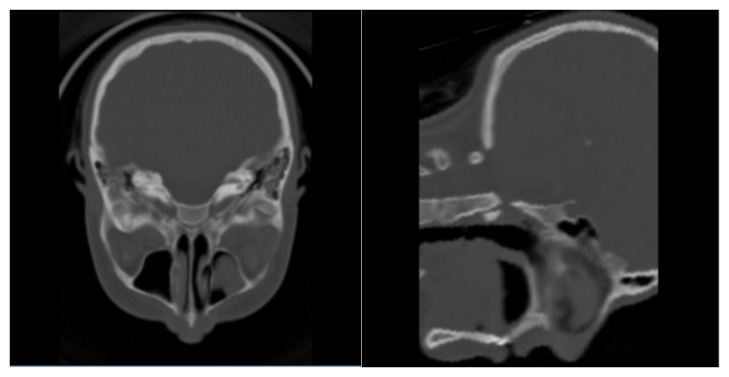
\includegraphics[scale=0.56]{1.pdf}
\end{figure}

\section{Iso-surface rendering}
When you choose Iso-surface rendering, you need to track the ray direction to find the first hit postion and composite the color and opacity from hit position. 
\begin{lstlisting}
//data access to scalar value in 3D valume texture
vec4 value = texture3D(vol_texture, position);
scalar = value.a;
if (scalar >= iso_value && !flag)
{
	flag = 1;
	hit_pos = position;
}
\end{lstlisting}

\begin{figure}[!htb]
\centering
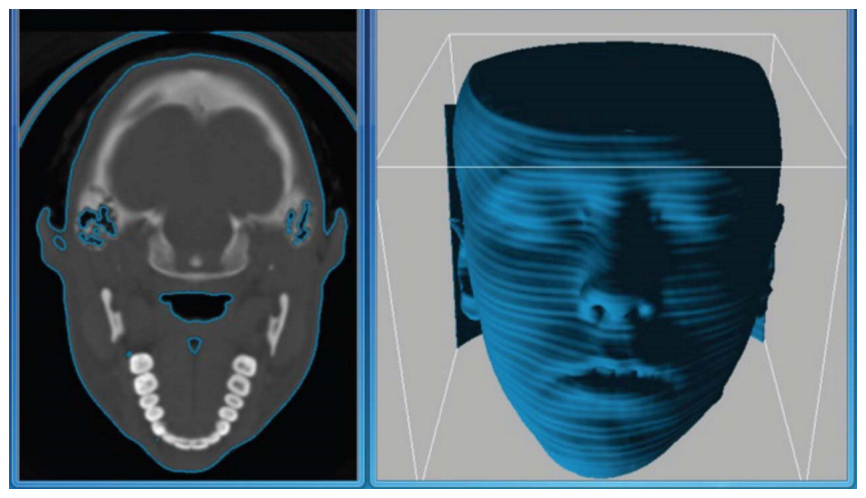
\includegraphics[scale=0.70]{2.pdf}
\end{figure}

\section{Bonus}
\subsection*{1. Axis-aligned Clipping planes}
In order to clip plane, I don't track the ray direction from the entry position, instead using modified position in the plane. 
\begin{lstlisting}
//clip plane
position = position + 200 * raydir * step_size;
\end{lstlisting}

\begin{figure}[!htb]
\centering
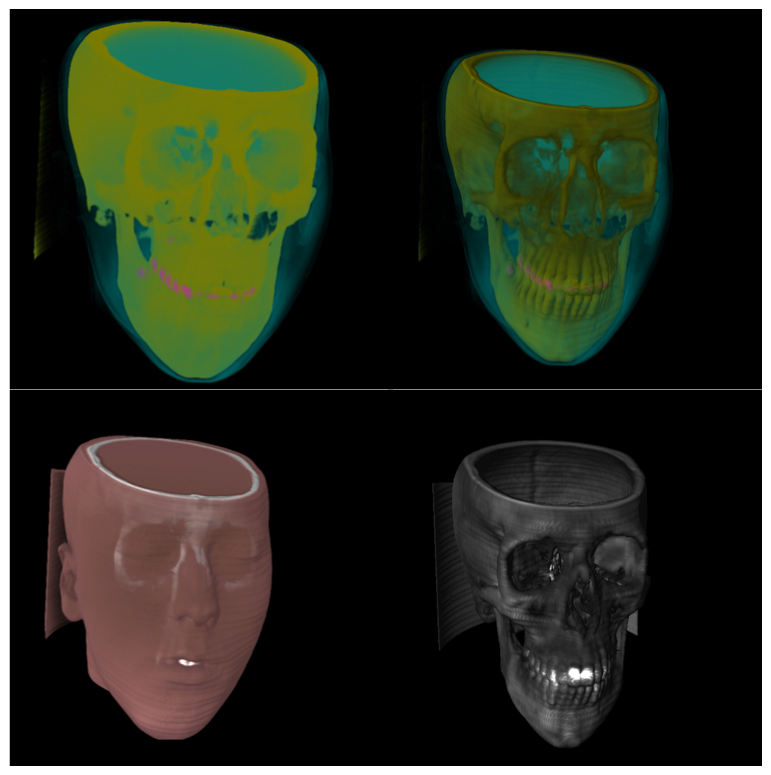
\includegraphics[scale=0.70]{3.pdf}
\end{figure}


\subsection*{2. maximum Intensity Projection}
Instead of transfer integration, maximum intensity projection means only choose the maximum intensity along each ray direction.
\begin{lstlisting}
//Maximum intensity projection
if (scalar > max_scalar)
{
	MIP = value;
	max_scalar = scalar;
}
...
gl_FragColor = (vec4(ambi + diffuse + spec, 1.0)) * MIP;
\end{lstlisting}


			
\begin{figure}[!htb]
\centering
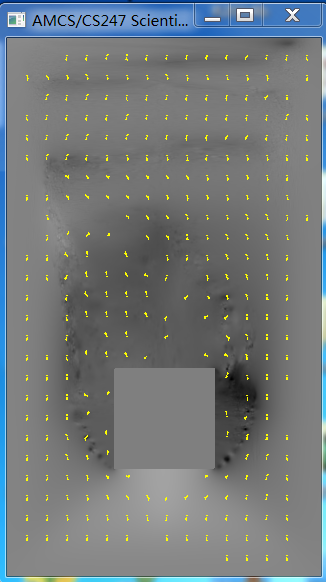
\includegraphics[scale=0.60]{4.pdf}
\end{figure}
%%%%%%%%%%%%%%%%%%%%%%%%%%%%%%%%%%%%%%%%%%%    REFERENCES
%\clearpage
%\singlespacing
%\bibliographystyle{plainnat}
%\bibliography{filename} % Name of .bib references file
%\clearpage

%\vspace{3cm}

%%%%%%%%%%%%%%%%%%%%%%%%%%%%%%%%%%%%%%%%%%%    TABLES & FIGURES
%\newpage
%\section{Tables and Figures}\label{sec:tables}


%%%%%%%%%%%%%%%%%%%%%%%%%%%%%%%%%%%%%%%%%%%    APPENDIX
%\newpage
%\appendix
%\section{Appendix}\label{sec:appendix}


\end{document}
